\section{The Non deterministic Constraint Logic Model of
Computation}
\label{sec:NCL}
The NCL machine can be viewed as a framework for proving PSPACE hardness. It can be seen as a model of computation that captures the class PSPACE. The machine notion will be formulated using a graph notation as described below.  

\subsection{Graph formulation}
The NCL machine can be interpreted as an undirected graph $G = (V,E)$ where to each edge is assigned a weight $w : E \rightarrow \mathbb{Z^+}$ and to each vertex is assigned an integer to represent its minimum inflow. 

\begin{defn}
A configuration using the graph formulation given above is an orientation of its edges such that it satisfies the following constraint : 
\begin{enumerate}
    \item  The sum of all in-degree edges at each vertex must be at least the minimum inflow of the vertex. This constraint is called the minimum inflow constraint.
\end{enumerate}
\end{defn}

\begin{defn}
A reconfiguration step from one configuration to the other is simply the reversal of an edge at a time such that the minimum inflow constraint remains satisfiable. 
\end{defn}

\begin{defn}
A constraint graph is a directed graph satisfying the minimum inflow constraint.
\end{defn}

\begin{defn}
A constraint graph is in normal form if it is a cubic graph and all edges weights $\in \{1,2\}$. The weights may also be represented graphically by drawing edges of weight one as red and edges of weight two as blue. The minimum inflow constraint for each vertex is set to $2$. Additionally each vertex should be incident to an even number of red edges. 

This type of constraint graph is also called and/or constraint graph and will be referred to as such in the following sections. 
\end{defn}

\subsection{Circuit formulation}
And/or constraint graphs are called as such because the two possible type of vertices behave like an AND gate and an OR gate in Boolean logic. 

\begin{figure}[H]
\centering
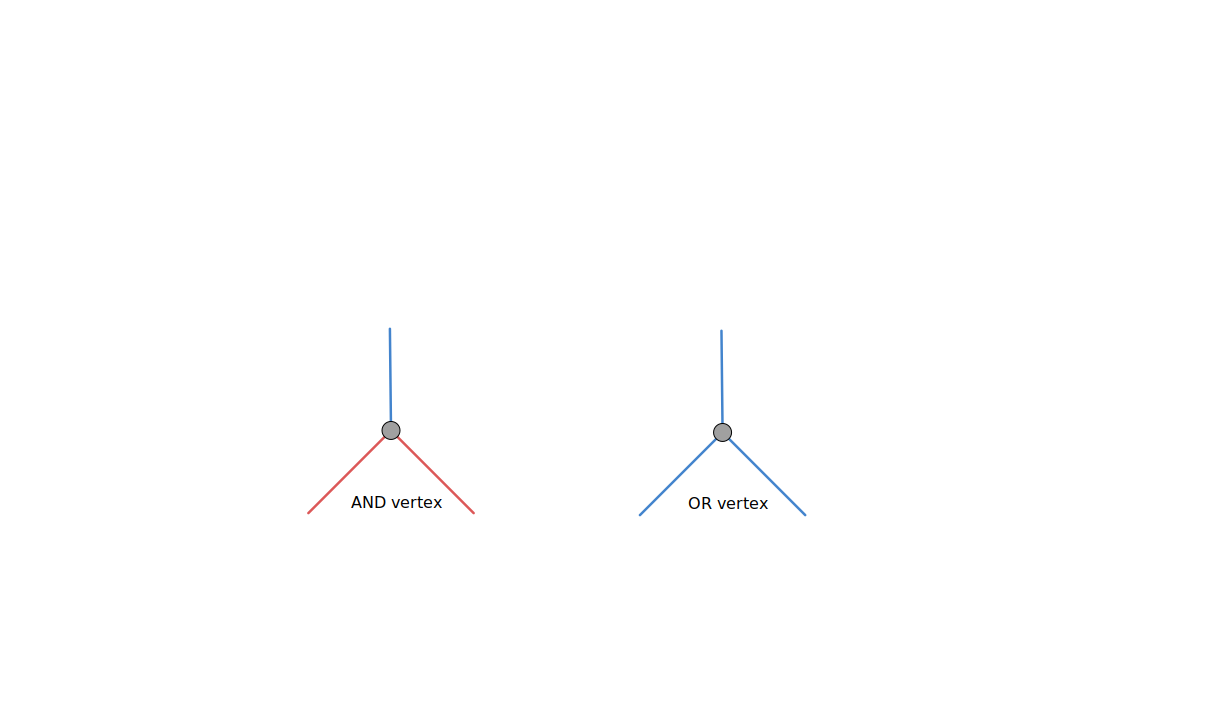
\includegraphics[width=0.35\textwidth]{res/andOrVertex.pdf}
\caption{left image: AND vertex     right image : OR vertex}
\label{fig:circle}
\end{figure}

A vertex with two red edges and one blue edge behaves like an AND gate because it requires both red edges to point inwards before the blue edge can be made to point outwards. 
\begin{figure}[H]
\centering
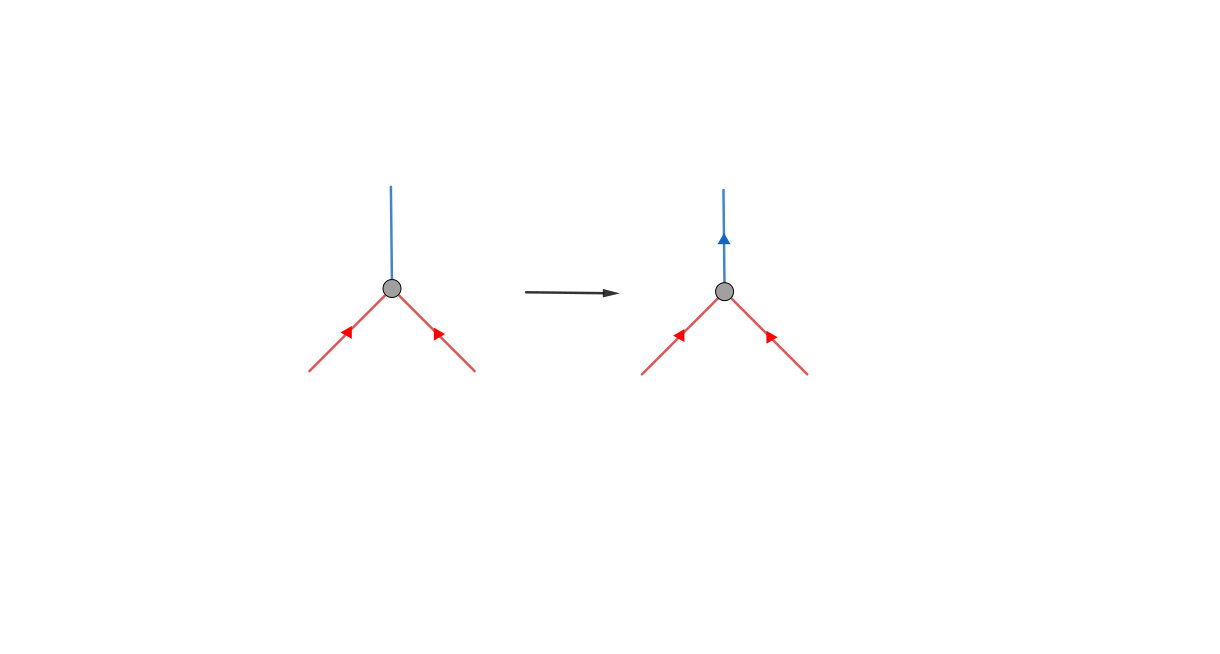
\includegraphics[width=0.35\textwidth]{res/andVertex.pdf}
\caption{Activation of the output edge when the two input edges are activated}
\label{fig:circle}
\end{figure}

A vertex with three blue edges behaves like an OR gate, since it requires at least one input edge to point inwards before the output edge can be activated.
\begin{figure}[H]
\centering
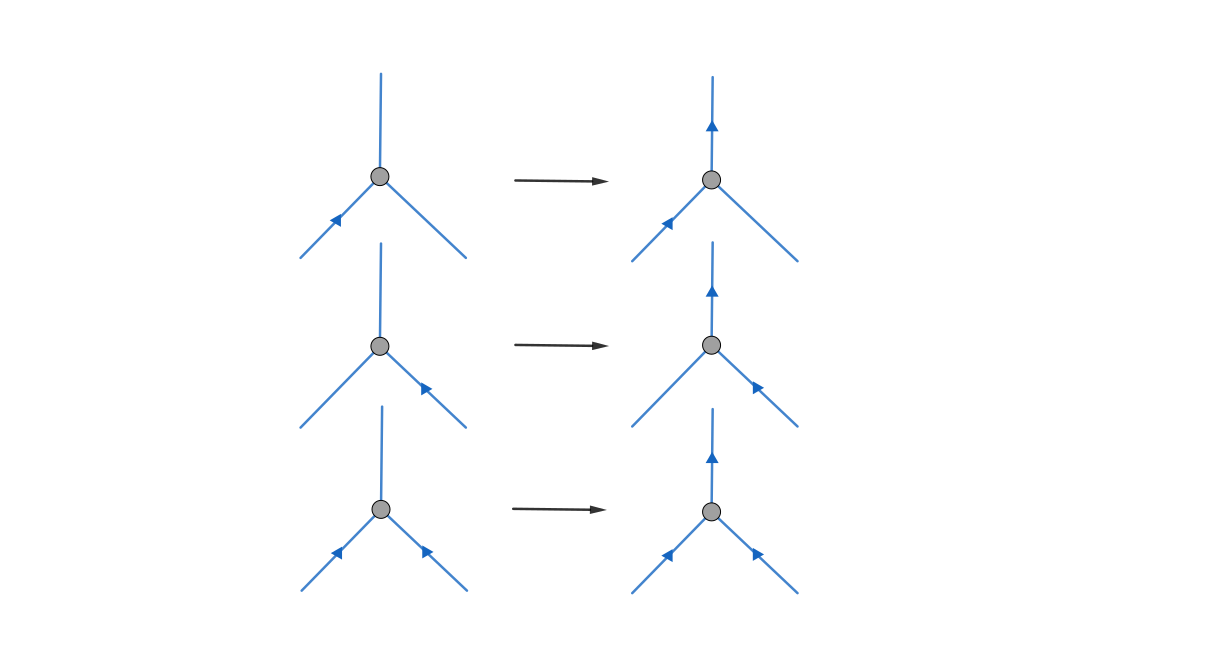
\includegraphics[width=0.35\textwidth]{res/orVertex.pdf}
\caption{Different behaviours of an OR vertex}
\label{fig:circle}
\end{figure}

\begin{defn}
Activation of an edge :  
\begin{enumerate}
    \item An input edge is active when it is an incoming edge. 
    \item An output edge is active when it is an outgoing edge.
\end{enumerate}
\end{defn}

\begin{defn}
Two decision problems arise regarding the graph formulation of the  NCL machine. 
\begin{enumerate}
    \item Given the and/or constraint graph, can a specified edge be eventually reversed by a sequence of reconfiguration steps ?
    \item Given two satisfying configurations, is one configuration reachable to the other by a single edge reversal at a time? 
\end{enumerate}
The answer to both questions happens to be PSPACE-complete. 
In this work a proof sketch is given for the second question.
\end{defn}

\subsection{PSPACE-completeness}

\subsubsection{NCL is PSPACE-hard}
\begin{proof}
The PSPACE-hardness of NCL is proved by doing a reduction from QBF problem, a well known PSPACE-complete problem. The goal of this reduction is to translate a given Quantified Boolean Formula $\phi$ into an instance of NCL so that the result gate in the resulting circuit may be activated if and only if $\phi$ is true. 

\begin{defn}
QBF is the generalized satisfiability problem that includes universal ($\forall$) and existential $(\exists)$ quantifiers. A QBF formula is a Boolean formula containing quantifiers. 
\end{defn}

\paragraph{QBF $\leq_p$ NCL} \hfill \break

\begin{figure}[H]
\centering
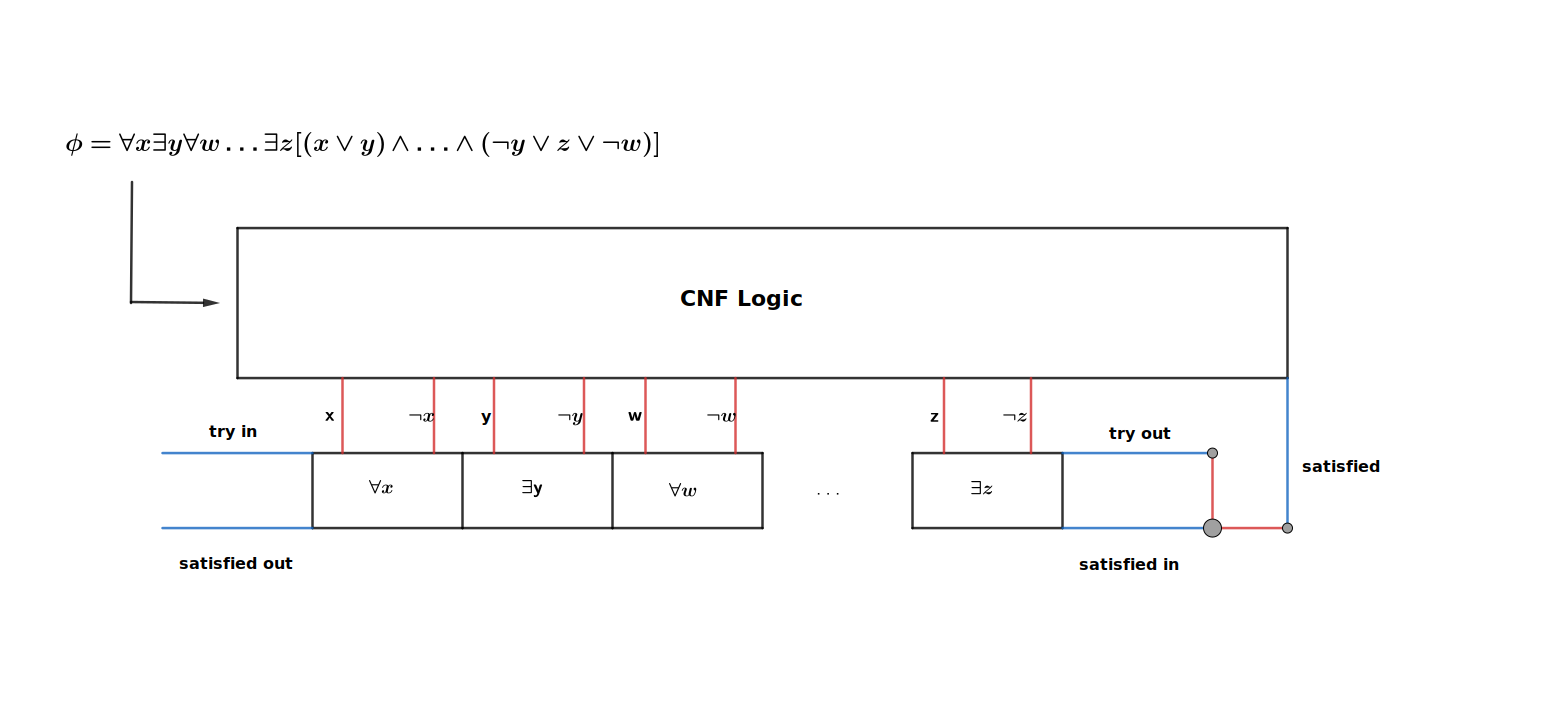
\includegraphics[width=0.9\textwidth]{res/NCL.pdf}
\caption{Schematic of the reduction from Quantified Boolean Formulas to NCL}
\label{fig:circle}
\end{figure}

The reduction from QBF to NCL to prove the PSPACE-hardness is given in the following steps : 
\begin{enumerate}
    \item Compute the and/or constraint graph of the unquantified formula ($[(x \vee y) \wedge \dots \wedge (\neg y \vee z \vee \neg w)]$) which will referred to as the CNF netork. This problem is 
    $\mathcal{NP}-complete$\cite{goos_nondeterministic_2002}.
    \item Associate a quantifier gadget to each quantifier variable in the formula($\forall x \exists y \forall w \dots \exists z$). Each quantifier gadget is connected together.
    \item Associate a variable gadget to represent each variable in the formula. 
    \item Connect each quantifier gadget to its corresponding variable gadget. The orientation of each edge designates which variable is assigned to true or false.  
    \item The variable gadgets are then fed into the CNF network. 
    \item The output of the CNF network is connected to the rightmost quantifier gadget through an AND vertex. 
    \item The output of the overall circuit comes through the satisfied out port from the leftmost quantifier gadget. 
\end{enumerate}

\paragraph{The gadgets in more detail} \hfill \break
\begin{enumerate}
   \item Existential quantifier gadget.
   \begin{figure}[H]
    \centering
    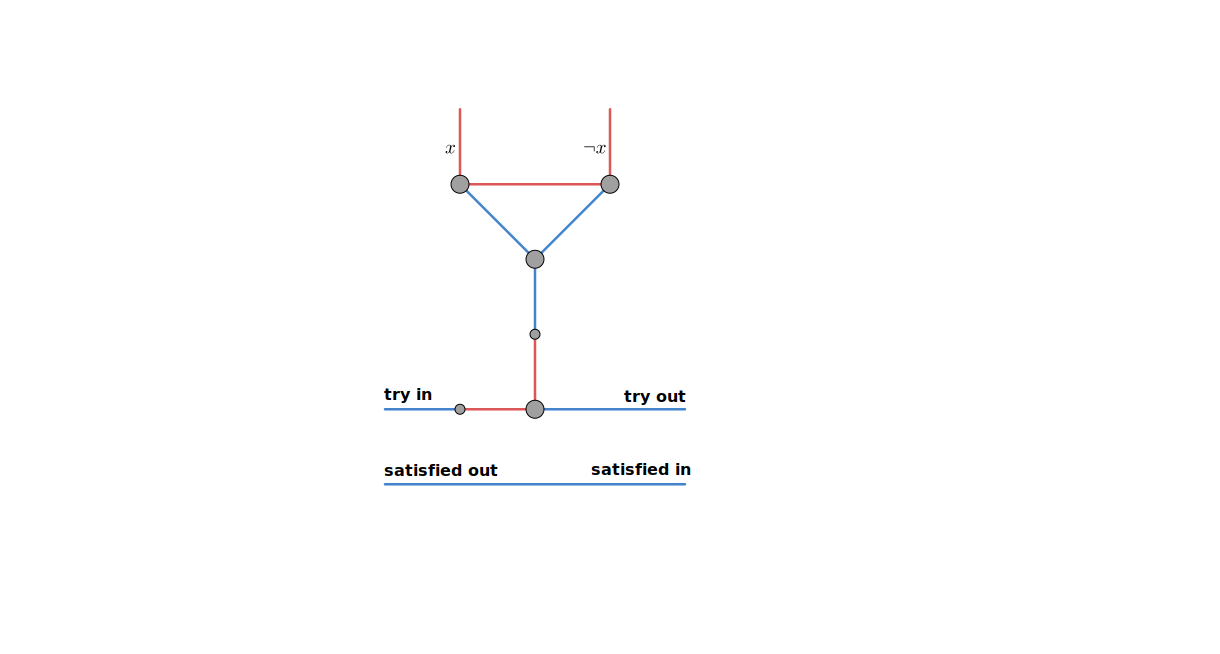
\includegraphics[width=0.3\textwidth]{res/existential.pdf}
    \caption{Existential gadget}
    \label{fig:circle}
    \end{figure}
    
    \begin{enumerate}
        \item The try in edge is considered as the input edge.
        \item The try out edge is considered as the output edge. 
        \item The top part of the existential gadget is called a latch. \\
        The latch is in locked state when its designated output edge is activated. It is called locked state because when the output edge is activated no other edge in the latch can change orientation.
        
        \begin{figure}[H]
        \centering
        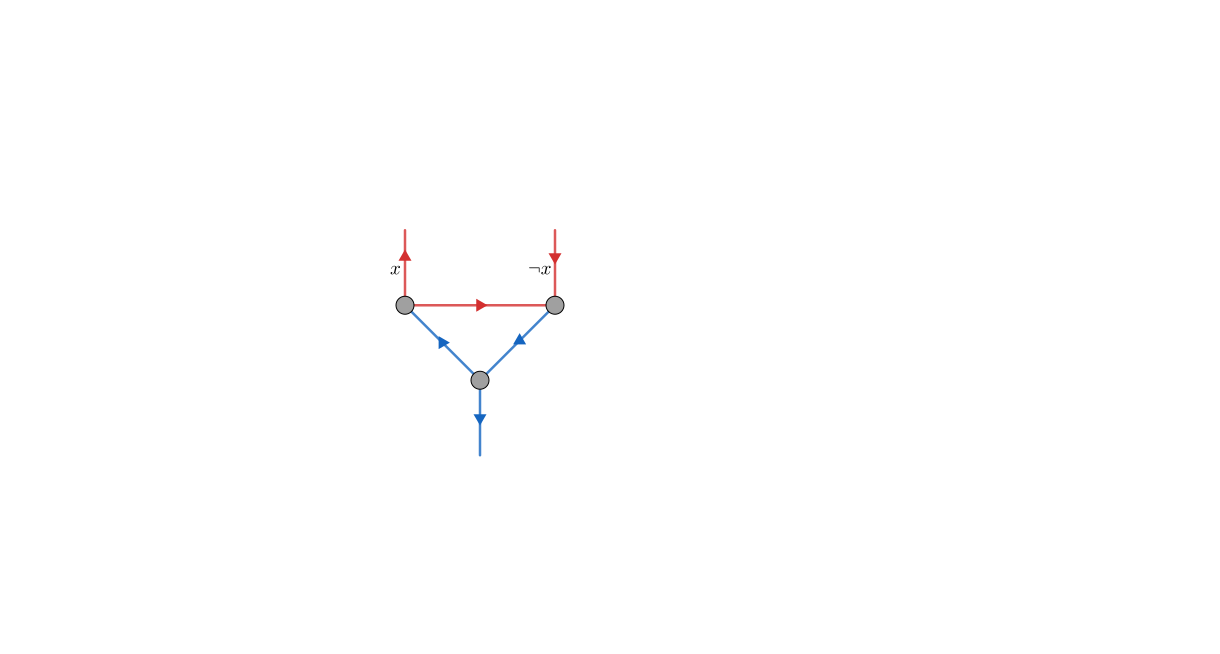
\includegraphics[width=0.2\textwidth]{res/existential2.pdf}
        \caption{Latch}
        \label{fig:circle}
        \end{figure}

        \begin{example}
        If the designated output port is the edge $(1)$ and it points downwards, it prevents other edges from changing orientation. For instance edge $(2)$ cannot flip, which then prevents edges $(3)$ and $(4)$ from reversing. Thus edge $(5)$ cannot point inwards either. Only edge $(6)$ can reverse. 
        
        \begin{figure}[H]
        \centering
        \includegraphics[width=0.2\textwidth]{res/existential3.pdf}
        \caption{Locked state}
        \label{fig:existential3}
        \end{figure}
        \end{example}
        
        \item The latch is then connected to the bottom part of the existential gadget through an edge converter which converts edge $(1)$ from a red edge to a blue edge. (the details about the edge converter gadget is omitted here. Refer to \cite{goos_nondeterministic_2002} for more details). \\
        
        In summary the existential gadget works as follows : 
        It receives a signal from the previous quantifier gadget to assign a value to its variable. Once the variable value is locked, edge ($6$) in figure \ref{fig:existential3} points out, activating the red edge.Thus allowing the try out edge to activate and signal the next quantifier gadget to do the same process. If the later reports back with a positive answer, the current gadget returns the answer back to its caller.  
        
        \begin{figure}[H]
        \centering
        \includegraphics[width=0.3\textwidth]{res/existential1.pdf}
        \caption{Universal quantifier gadget signaled to assign a value to its variable and to signal the next quantifier to do the same}
        \label{fig:circle}
        \end{figure}
    
    \end{enumerate}
    
    \item Universal quantifier gadget. \\ 
    The universal quantifier has a slightly more complex structure than the existential quantifier. 
    There are two latches in the universal gadget. Both whose edges are connected to an AND gate. As earlier the latches play the role of a one bit memory since their locking mechanism allows the assignment of the different variables to true or false. The satisfied out edge is activated only when both latches are in locked in state i.e when the assignments are successful. 
    
    \begin{figure}[H]
    \centering
    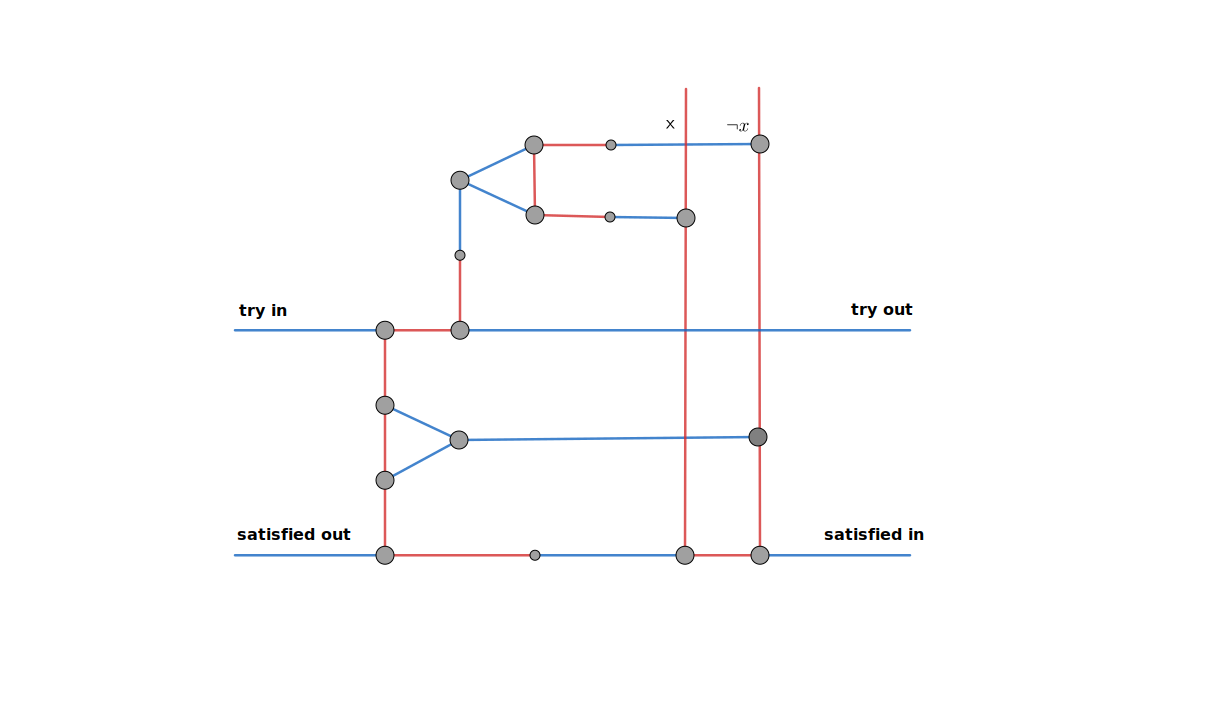
\includegraphics[width=0.7\textwidth]{res/universal.pdf}
    \caption{Universal quantifier gadget}
    \label{fig:circle}
    \end{figure}
    
    \item The variable gadget \\
    The variable gadget is none other than the latches encountered in the universal and existential gadgets.
\end{enumerate}

\paragraph{The general workflow} \hfill \break

Once the CNF network is computed, the result comes through the satisfied edge. The satisfied edge is activated if and only if the CNF formula is satisfied. 
Once all the variables are set, the try out edge is activated as well which then allows edges $(1)$ and $(2)$ to activate leading to the activation of the satisfied in edge. 
   
    \begin{figure}[H]
    \centering
    \includegraphics[width=0.9\textwidth]{res/NCL1.pdf}
    \caption{Schematic of the reduction from Quantified Boolean Formulas to NCL}
    \label{fig:circle}
    \end{figure}
    
This, then activates the quantifier gadgets leading to the activation of the satisfied out edge if and only if $\phi$ is satisfied.   

\begin{lemma}\cite{goos_nondeterministic_2002}
A quantifier gadget${^'}$s satisfied in port may not activate unless its try out port is active.
\end{lemma}

\begin{lemma}\cite{goos_nondeterministic_2002}
An existential quantifier gadget may activate its satisfied out port if and only if its satisfied in port is active with its variable locked in some state.
\end{lemma}

\begin{lemma} \cite{goos_nondeterministic_2002}
A universal quantifier gadget may activate its satisfied out port if and only if its satisfied in port is at one time active with its variable locked in the false (x) state, and at a later time is again active with its variable locked in
the true (x) state, with try in remaining active throughout.
\end{lemma}

\begin{lemma} \cite{goos_nondeterministic_2002}
A quantifier gadget may activate its satisfied out port if and only if its try in port is active, and the formula read from the corresponding quantifier to the right is true given the variable assignments that are fixed by the quantifier
gadgets to the left.
\end{lemma}

\begin{theorem}
NCL is PSPACE-complete
\cite{goos_nondeterministic_2002}
\end{theorem}

\end{proof}